\chapter{Pruebas}

En este capítulo se describe la estrategia de verificación adoptada para validar que el sistema desarrollado cumple con los requisitos especificados y con los flujos de interacción definidos en el análisis. El objetivo es demostrar que el videojuego se comporta de forma correcta y estable ante las distintas situaciones que pueden producirse durante su uso. La batería de pruebas se organiza en ocho bloques temáticos que cubren los requisitos funcionales y no funcionales, e incluye adicionalmente una sección dedicada a la usabilidad percibida por usuarios reales durante sesiones de juego supervisadas.

% ─────────────────────────────────────────────────────────────────────────────
\section{Enfoque de pruebas}
% ─────────────────────────────────────────────────────────────────────────────

En un entorno de desarrollo profesional, la verificación de un sistema software de esta naturaleza se abordaría mediante una estrategia de pruebas automatizadas estructurada en varios niveles. Las pruebas unitarias verificarían de forma aislada cada componente lógico del sistema, como el motor de reglas de movimiento o el sistema de resolución de combates, comprobando que producen el resultado esperado ante un conjunto exhaustivo de entradas. Las pruebas de integración validarían la interacción correcta entre componentes, asegurando por ejemplo que el controlador de input delega adecuadamente en el tablero y que este actualiza el estado de la partida de forma consistente. Finalmente, las pruebas de sistema o de extremo a extremo ejercitarían flujos completos de usuario, desde el despliegue inicial hasta la condición de victoria, simulando el comportamiento real del jugador. Herramientas como \textit{NUnit} o \textit{xUnit} en el ecosistema .NET, combinadas con un pipeline de integración continua, permitirían ejecutar esta batería de forma automática ante cada cambio en el código, detectando regresiones de manera inmediata.

\clearpage

Dado el carácter académico e individual del proyecto y las restricciones temporales inherentes a un TFG, la automatización completa de las pruebas queda fuera del alcance definido. No obstante, la arquitectura adoptada, con la lógica del videojuego separada en clases C\# puras e independientes del motor, facilita que dichas pruebas automatizadas puedan incorporarse en el futuro sin necesidad de modificar el código de producción. En su lugar, se ha llevado a cabo una batería de pruebas de aceptación organizadas por bloques temáticos, cubriendo todos los requisitos funcionales y no funcionales identificados en el análisis. Cada prueba define de forma explícita su precondición, la acción ejecutada y el resultado esperado, lo que permite reproducirlas de manera sistemática y trazarlas directamente con los requisitos del sistema.

% ─────────────────────────────────────────────────────────────────────────────
\section{Batería de pruebas}
% ─────────────────────────────────────────────────────────────────────────────

En este apartado se recoge el conjunto de pruebas funcionales realizadas sobre el sistema para verificar que el comportamiento del videojuego se ajusta a los requisitos especificados y a los flujos descritos en los casos de uso. Las pruebas se organizan por bloques temáticos y se presentan en formato tabular, indicando para cada caso la precondición, los pasos ejecutados, el resultado esperado y si la prueba ha sido superada.

\subsection{Bloque 1 — Despliegue inicial}

\begin{table}[H]
	\centering
	\small
	\begin{tabular}{|>{\centering\arraybackslash}p{1cm}|>{\centering\arraybackslash}p{4cm}|>{\centering\arraybackslash}p{4cm}|>{\centering\arraybackslash}p{4cm}|>{\centering\arraybackslash}p{1.5cm}|}
		\hline
		\textbf{ID} & \textbf{Descripción} & \textbf{Precondición} & \textbf{Resultado esperado} & \textbf{¿Pasa?} \\
		\hline
		PR-01 & Iniciar una nueva partida desde el menú principal & El sistema muestra el menú principal & El tablero se inicializa y se muestra la interfaz de despliegue & \cellcolor{green!40}Sí \\
		\hline
		PR-02 & Intentar comenzar la partida sin colocar todas las piezas & Pantalla de despliegue activa & El sistema impide el inicio y permanece en la fase de despliegue & \cellcolor{green!40}Sí \\
		\hline
		PR-03 & Colocar una pieza fuera de la zona de despliegue permitida & Pantalla de despliegue activa & El sistema rechaza la acción y no coloca la pieza & \cellcolor{green!40}Sí \\
		\hline
		PR-04 & Intentar colocar dos piezas en la misma casilla & Al menos una pieza ya colocada & El sistema quita la pieza original & \cellcolor{green!40}Sí \\
		\hline
		PR-05 & Colocar todas las piezas y confirmar inicio & Todas las piezas del jugador colocadas & El bot despliega sus piezas y comienza el turno del jugador & \cellcolor{green!40}Sí \\
		\hline
	\end{tabular}
	\caption{Pruebas del bloque 1: Despliegue inicial}
\end{table}

\clearpage

\subsection{Bloque 2 — Movimiento}

\begin{table}[H]
	\centering
	\small
	\begin{tabular}{|>{\centering\arraybackslash}p{1cm}|>{\centering\arraybackslash}p{4cm}|>{\centering\arraybackslash}p{4cm}|>{\centering\arraybackslash}p{4cm}|>{\centering\arraybackslash}p{1.5cm}|}
		\hline
		\textbf{ID} & \textbf{Descripción} & \textbf{Precondición} & \textbf{Resultado esperado} & \textbf{¿Pasa?} \\
		\hline
		PR-06 & Seleccionar una pieza propia con movimientos disponibles & Turno del jugador activo & Las casillas de destino válidas quedan resaltadas & \cellcolor{green!40}Sí \\
		\hline
		PR-07 & Seleccionar una pieza propia sin movimientos disponibles & Turno del jugador activo & No se resalta ninguna casilla ni se registra selección & \cellcolor{green!40}Sí \\
		\hline
		PR-08 & Hacer clic fuera de una casilla válida tras seleccionar una pieza & Pieza seleccionada con casillas resaltadas & Se cancela la selección y se eliminan los resaltados & \cellcolor{green!40}Sí \\
		\hline
		PR-09 & Mover una pieza a una casilla vacía válida & Pieza seleccionada y casilla resaltada & La pieza se desplaza a la casilla y el turno pasa al bot & \cellcolor{green!40}Sí \\
		\hline
		PR-10 & Intentar mover una pieza a una casilla intransitable & Turno del jugador activo & El sistema impide el movimiento; la casilla no aparece resaltada & \cellcolor{green!40}Sí \\
		\hline
		PR-11 & Intentar mover una pieza a una casilla ocupada por otra pieza propia & Turno del jugador activo & El sistema no permite el movimiento; la casilla no está resaltada & \cellcolor{green!40}Sí \\
		\hline
		PR-12 & Mover el Explorador más de una casilla en línea recta & Turno del jugador, Explorador disponible & La pieza se desplaza y su identidad queda revelada permanentemente & \cellcolor{green!40}Sí \\
		\hline
		PR-13 & Mover el Explorador exactamente una casilla & Turno del jugador, Explorador disponible & La pieza se desplaza sin revelar su identidad & \cellcolor{green!40}Sí \\
		\hline
		PR-14 & Intentar realizar una acción durante el turno del bot & Turno del bot en ejecución & El sistema ignora el input del jugador & \cellcolor{green!40}Sí \\
		\hline
	\end{tabular}
	\caption{Pruebas del bloque 2: Movimiento}
\end{table}

\clearpage

\subsection{Bloque 3 — Combate}

\begin{table}[H]
	\centering
	\small
	\begin{tabular}{|>{\centering\arraybackslash}p{1cm}|>{\centering\arraybackslash}p{4cm}|>{\centering\arraybackslash}p{4cm}|>{\centering\arraybackslash}p{4cm}|>{\centering\arraybackslash}p{1.5cm}|}
		\hline
		\textbf{ID} & \textbf{Descripción} & \textbf{Precondición} & \textbf{Resultado esperado} & \textbf{¿Pasa?} \\
		\hline
		PR-15 & Pieza de mayor rango ataca a pieza de menor rango & Ambas piezas en posiciones adyacentes válidas & La pieza atacante ocupa la casilla; la defensora es eliminada & \cellcolor{green!40}Sí \\
		\hline
		PR-16 & Pieza de menor rango ataca a pieza de mayor rango & Ambas piezas en posiciones adyacentes válidas & La pieza atacante es eliminada; la defensora permanece & \cellcolor{green!40}Sí \\
		\hline
		PR-17 & Dos piezas del mismo rango se enfrentan & Ambas piezas en posiciones adyacentes válidas & Empate: ambas piezas son eliminadas del tablero & \cellcolor{green!40}Sí \\
		\hline
		PR-18 & Saboteador ataca a una Torreta & Saboteador y Torreta en posiciones adyacentes & El Saboteador vence y ocupa la casilla de la Torreta & \cellcolor{green!40}Sí \\
		\hline
		PR-19 & Pieza distinta al Saboteador ataca a una Torreta & Pieza no-Saboteador y Torreta adyacentes & La pieza atacante es destruida; la Torreta permanece & \cellcolor{green!40}Sí \\
		\hline
		PR-20 & Phantom ataca a la Máquina de guerra & Phantom y Máquina de guerra en posiciones adyacentes & El Phantom vence independientemente del rango & \cellcolor{green!40}Sí \\
		\hline
		PR-21 & Pieza distinta al Phantom ataca a la Máquina de guerra & Pieza no-Phantom y Máquina de guerra adyacentes & El combate se resuelve por rango numérico según las reglas normales & \cellcolor{green!40}Sí \\
		\hline
		PR-22 & Combate entre dos piezas, al menos una oculta & Una o ambas piezas con identidad no revelada & Ambas identidades quedan reveladas y permanecen visibles & \cellcolor{green!40}Sí \\
		\hline
		PR-23 & Pieza ya revelada entra en un nuevo combate & Pieza previamente revelada en partida & La pieza sigue mostrando su identidad correctamente & \cellcolor{green!40}Sí \\
		\hline
		PR-24 & La interfaz de combate se muestra y cierra correctamente & Se produce un combate durante un turno & Se muestra la pantalla de resolución; al confirmar, se cierra y el juego continúa & \cellcolor{green!40}Sí \\
		\hline
	\end{tabular}
	\caption{Pruebas del bloque 3: Combate}
\end{table}

\clearpage

\subsection{Bloque 4 — Condiciones de victoria}

\begin{table}[H]
	\centering
	\small
	\begin{tabular}{|>{\centering\arraybackslash}p{1cm}|>{\centering\arraybackslash}p{4cm}|>{\centering\arraybackslash}p{4cm}|>{\centering\arraybackslash}p{4cm}|>{\centering\arraybackslash}p{1.5cm}|}
		\hline
		\textbf{ID} & \textbf{Descripción} & \textbf{Precondición} & \textbf{Resultado esperado} & \textbf{¿Pasa?} \\
		\hline
		PR-25 & El jugador destruye el Núcleo de energía del bot & Partida en curso, Núcleo rival accesible & La partida termina inmediatamente y el jugador gana & \cellcolor{green!40}Sí \\
		\hline
		PR-26 & El bot destruye el Núcleo de energía del jugador & Partida en curso, Núcleo del jugador accesible & La partida termina inmediatamente y el jugador pierde & \cellcolor{green!40}Sí \\
		\hline
		PR-27 & Todas las piezas móviles del jugador son eliminadas & Partida en curso & El sistema detecta que el jugador no puede mover y declara su derrota & \cellcolor{green!40}Sí \\
		\hline
		PR-28 & Todas las piezas móviles del bot son eliminadas & Partida en curso & El sistema detecta que el bot no puede mover y declara la victoria del jugador & \cellcolor{green!40}Sí \\
		\hline
		PR-29 & El jugador y el bot se quedan sin piezas moviles en el mismo turno & Partida en curso & La pantalla de fin de partida aparece indicando un empate & \cellcolor{green!40}Sí \\
		\hline
		PR-30 & El jugador selecciona jugar otra partida desde la pantalla de fin & Pantalla de fin de partida visible & El sistema reinicia completamente el estado y vuelve a la fase de despliegue & \cellcolor{green!40}Sí \\
		\hline
		PR-31 & El jugador selecciona volver al menú principal desde la pantalla de fin & Pantalla de fin de partida visible & El sistema navega al menú principal & \cellcolor{green!40}Sí \\
		\hline
	\end{tabular}
	\caption{Pruebas del bloque 4: Condiciones de victoria}
\end{table}

\clearpage

\subsection{Bloque 5 — Interfaz y feedback visual/sonoro}

\begin{table}[H]
	\centering
	\small
	\begin{tabular}{|>{\centering\arraybackslash}p{1cm}|>{\centering\arraybackslash}p{4cm}|>{\centering\arraybackslash}p{4cm}|>{\centering\arraybackslash}p{4cm}|>{\centering\arraybackslash}p{1.5cm}|}
		\hline
		\textbf{ID} & \textbf{Descripción} & \textbf{Precondición} & \textbf{Resultado esperado} & \textbf{¿Pasa?} \\
		\hline
		PR-32 & Sonido de movimiento al desplazar una pieza & Turno del jugador, pieza movida a casilla vacía & Se reproduce el efecto de sonido asociado al movimiento & \cellcolor{green!40}Sí \\
		\hline
		PR-33 & Sonido de combate al producirse un enfrentamiento & Combate iniciado durante cualquier turno & Se reproduce el efecto de sonido asociado al combate & \cellcolor{green!40}Sí \\
		\hline
		PR-34 & Sonido de navegación por menús & Usuario navega entre menús & Se reproducen los efectos sonoros asociados a los botones & \cellcolor{green!40}Sí \\
		\hline
		PR-35 & Toda la interacción es posible exclusivamente con el ratón & El videojuego está en cualquier estado & Ninguna acción requiere el uso del teclado & \cellcolor{green!40}Sí \\
		\hline
	\end{tabular}
	\caption{Pruebas del bloque 5: Interfaz y feedback}
\end{table}

\clearpage

\subsection{Bloque 6 — Menús y navegación}

\begin{table}[H]
	\centering
	\small
	\begin{tabular}{|>{\centering\arraybackslash}p{1cm}|>{\centering\arraybackslash}p{4cm}|>{\centering\arraybackslash}p{4cm}|>{\centering\arraybackslash}p{4cm}|>{\centering\arraybackslash}p{1.5cm}|}
		\hline
		\textbf{ID} & \textbf{Descripción} & \textbf{Precondición} & \textbf{Resultado esperado} & \textbf{¿Pasa?} \\
		\hline
		PR-36 & Pausar la partida en mitad de un turno del jugador & Turno del jugador activo & El menú de pausa se abre y la partida queda pausado & \cellcolor{green!40}Sí \\
		\hline
		PR-37 & Reanudar la partida desde el menú de pausa & Menú de pausa abierto & La partida continúa desde el mismo estado en que fue pausada & \cellcolor{green!40}Sí \\
		\hline
		PR-38 & Abandonar la partida desde el menú de pausa & Menú de pausa abierto & El sistema navega al menú principal sin errores & \cellcolor{green!40}Sí \\
		\hline
		PR-39 & Consultar las reglas desde el menú principal & Sistema en el menú principal & Se muestra el menú de reglas completo con toda la información & \cellcolor{green!40}Sí \\
		\hline
		PR-40 & Consultar las reglas desde el menú de pausa & Menú de pausa abierto & Se muestra el menú de reglas; al cerrarlo, el sistema regresa al menú de pausa & \cellcolor{green!40}Sí \\
		\hline
		PR-41 & Ajustar el volumen de las pistas de sonido desde el menú de opciones & Menú de opciones accesible & El cambio se aplica inmediatamente y se mantiene durante la sesión & \cellcolor{green!40}Sí \\
		\hline
		PR-42 & Acceder al menú de opciones desde el menú principal & Sistema en el menú principal & El menú de opciones se abre correctamente & \cellcolor{green!40}Sí \\
		\hline
		PR-43 & Acceder al menú de opciones desde el menú de pausa & Menú de pausa abierto & El menú de opciones se abre; al cerrarlo regresa al menú de pausa & \cellcolor{green!40}Sí \\
		\hline
	\end{tabular}
	\caption{Pruebas del bloque 6: Menús y navegación}
\end{table}

\clearpage

\subsection{Bloque 7 — Comportamiento del bot}

\begin{table}[H]
	\centering
	\small
	\begin{tabular}{|>{\centering\arraybackslash}p{1cm}|>{\centering\arraybackslash}p{4cm}|>{\centering\arraybackslash}p{4cm}|>{\centering\arraybackslash}p{4cm}|>{\centering\arraybackslash}p{1.5cm}|}
		\hline
		\textbf{ID} & \textbf{Descripción} & \textbf{Precondición} & \textbf{Resultado esperado} & \textbf{¿Pasa?} \\
		\hline
		PR-44 & El bot ejecuta su turno automáticamente tras el turno del jugador & El jugador ha completado su acción & El bot realiza un movimiento válido sin intervención del jugador & \cellcolor{green!40}Sí \\
		\hline
		PR-45 & El bot nunca se mueve a una casilla intransitable & Turno del bot activo & Ningún movimiento del bot aterriza en una casilla de tipo no-pasable & \cellcolor{green!40}Sí \\
		\hline
		PR-46 & El bot nunca ataca a sus propias piezas & Turno del bot activo & Todos los ataques del bot se dirigen a piezas del jugador & \cellcolor{green!40}Sí \\
		\hline
		PR-47 & El bot no actúa durante el turno del jugador & Turno del jugador activo & El bot permanece inactivo hasta que el jugador completa su acción & \cellcolor{green!40}Sí \\
		\hline
		PR-48 & El bot respeta las reglas especiales de combate & Turno del bot, situación con Torreta o Phantom & Los resultados de combate del bot siguen las mismas reglas especiales que las del jugador & \cellcolor{green!40}Sí \\
		\hline
	\end{tabular}
	\caption{Pruebas del bloque 7: Comportamiento del bot}
\end{table}

\clearpage

\subsection{Bloque 8 — Requisitos no funcionales}

\begin{table}[H]
	\centering
	\small
	\begin{tabular}{|>{\centering\arraybackslash}p{1cm}|>{\centering\arraybackslash}p{4cm}|>{\centering\arraybackslash}p{4cm}|>{\centering\arraybackslash}p{4cm}|>{\centering\arraybackslash}p{1.5cm}|}
		\hline
		\textbf{ID} & \textbf{Descripción} & \textbf{Precondición} & \textbf{Resultado esperado} & \textbf{¿Pasa?} \\
		\hline
		PR-49 & El videojuego arranca correctamente en Windows 10 & Ejecutable instalado en Windows 10 & El videojuego se inicia sin errores y llega al menú principal & \cellcolor{green!40}Sí \\
		\hline
		PR-50 & El videojuego arranca correctamente en Windows 11 & Ejecutable instalado en Windows 11 & El videojuego se inicia sin errores y llega al menú principal & \cellcolor{green!40}Sí \\
		\hline
		PR-51 & El videojuego funciona en un equipo con las especificaciones mínimas & Hardware mínimo: CPU doble núcleo 2,0~GHz, 8~GB RAM, GPU OpenGL~3.3 & El videojuego se ejecuta sin cuelgues, artefactos visuales ni caídas de rendimiento significativas & \cellcolor{green!40}Sí \\
		\hline
		PR-52 & Las acciones del jugador reciben respuesta en menos de 2 segundos & Videojuego en ejecución en condiciones normales & Ninguna acción provoca una espera superior a 2 segundos antes de que el sistema reaccione & \cellcolor{green!40}Sí \\
		\hline
		PR-53 & Un jugador sin experiencia identifica qué piezas puede mover sin consultar las reglas & Primera partida del jugador, sin leer el menú de reglas & El jugador es capaz de seleccionar y mover una pieza correctamente gracias al resaltado de casillas & \cellcolor{green!40}Sí \\
		\hline
	\end{tabular}
	\caption{Pruebas del bloque 8: Requisitos no funcionales}
\end{table}

\clearpage

% ─────────────────────────────────────────────────────────────────────────────
\section{Pruebas de usabilidad}
% ─────────────────────────────────────────────────────────────────────────────

Las pruebas de usabilidad tienen como objetivo evaluar en qué medida el videojuego resulta comprensible e intuitivo para usuarios que se enfrentan a él por primera vez, sin haber recibido instrucciones previas más allá de las que ofrece el propio sistema. A diferencia de las pruebas funcionales, que verifican la corrección del comportamiento del sistema, las pruebas de usabilidad miden la experiencia subjetiva del usuario y su capacidad para alcanzar los objetivos de juego de forma autónoma.

Se realizaron sesiones de prueba con varios usuarios de perfil distinto: 1 usuario sin experiencia en videojuegos de estrategia y 2 usuario con experiencia media o habitual en juegos de estrategia por turnos. En cada sesión se pidió al participante que realizara las siguientes tareas sin ayuda externa: iniciar una partida, desplegar todas sus piezas, completar al menos tres turnos de movimiento y combate, y navegar por el menú de reglas y el menú de pausa. Durante las sesiones se registraron los errores cometidos, los momentos de bloqueo y los comentarios verbales espontáneos de los participantes.

\begin{table}[H]
	\centering
	\small
	\begin{tabular}{|>{\centering\arraybackslash}p{1cm}|>{\centering\arraybackslash}p{4cm}|>{\centering\arraybackslash}p{3cm}|>{\centering\arraybackslash}p{5cm}|>{\centering\arraybackslash}p{1.5cm}|}
		\hline
		\textbf{ID} & \textbf{Descripción} & \textbf{Método} &
		\textbf{Resultado esperado} & \textbf{¿Pasa?} \\
		\hline
		PU-01 & El usuario comprende qué piezas puede mover sin leer las reglas &
		Observación directa en primera partida &
		El usuario selecciona una pieza propia y observa el resaltado de casillas
		disponibles sin bloqueos prolongados & \cellcolor{green!40}Sí \\
		\hline
		PU-02 & El usuario identifica cuándo es su turno y cuándo es el turno del bot &
		Observación directa &
		Ningún participante intenta realizar acciones durante el turno del bot & \cellcolor{green!40}Sí \\
		\hline
		PU-03 & El usuario comprende el resultado de un combate sin instrucciones &
		Observación y entrevista posterior &
		Todos los participantes describen correctamente el resultado tras presenciar
		la pantalla de resolución de combate & \cellcolor{green!40}Sí \\
		\hline
		PU-04 & El usuario es capaz de pausar la partida y retomar el juego &
		Observación directa &
		El participante localiza el botón de pausa y retoma la partida sin
		dificultad & \cellcolor{green!40}Sí \\
		\hline
		PU-05 & El usuario valora positivamente la claridad de la interfaz &
		Cuestionario post-sesión (escala 1--5) &
		Puntuación media igual o superior a 4 sobre 5 en apartado visual &
		\cellcolor{green!40}Sí \\
		\hline
	\end{tabular}
	\caption{Pruebas de usabilidad}
\end{table}

Los resultados de las sesiones fueron positivos en términos generales. El mecanismo de resaltado de casillas disponibles resultó ser el elemento más valorado, ya que permite al usuario descubrir las reglas de movimiento de forma inductiva sin necesidad de consultar la guía. El único punto de fricción recurrente fue la fase de despliegue inicial, donde el usuario sin experiencia tardó más tiempo en comprender cómo debía colocar todas las piezas antes de poder iniciar la partida. El botón de despliegue aleatorio indirectamente acabó ayudando en esa tarea, ya que los jugadores podrían utilizarlo por curiosidad y es entonces cuando verían que pueden quitar piezas, seleccionarlas a placer en la interfaz de despliegue y demás.

% ─────────────────────────────────────────────────────────────────────────────
\subsection{Cuestionario de evaluación}
% ─────────────────────────────────────────────────────────────────────────────

Con el objetivo de obtener una valoración más amplia y estructurada por parte de usuarios externos, se diseñó un cuestionario de evaluación distribuido a través de la plataforma Google Forms. Este instrumento permite recopilar datos cuantitativos y cualitativos sobre la percepción del software de manera estandarizada mediante la aplicación de preguntas binarias y escalas de valoración de cinco niveles ordenadas de mayor a menor grado de conformidad.

El cuestionario se organiza en seis bloques temáticos clave para evaluar la calidad del videojuego desde la perspectiva de la experiencia de usuario:
\begin{itemize}
	\item \textbf{Sonido:} Evalúa el uso del audio integrado, el nivel de agrado de las pistas musicales y los efectos, así como su impacto directo en la experiencia de juego.
	\item \textbf{Apartado visual:} Analiza el atractivo de la interfaz, la idoneidad de la paleta de colores seleccionada y la coherencia estética de los gráficos con la temática de ciencia ficción.
	\item \textbf{Operabilidad:} Mide la facilidad de uso de los controles, la claridad en la exposición de las reglas y la legibilidad de la tipografía y los textos informativos en pantalla.
	\item \textbf{Entretenimiento:} Cuantifica el grado de diversión percibido y la predisposición del usuario a recomendar el videojuego a terceros.
	\item \textbf{Inmersión:} Explora la capacidad del juego para capturar la atención inicial, la retención del usuario al finalizar la sesión y la alteración de la percepción del tiempo durante la partida.
	\item \textbf{Calificación global:} Recoge una valoración numérica general del proyecto en una escala del 1 al 10 y un apartado de observaciones abiertas para propuestas de mejora.
\end{itemize}

Los resultados cuantitativos obtenidos se muestran distribuidos en la Tabla~\ref{tab:resultados_encuesta_matriz}, mapeando de manera explícita la frecuencia de respuestas a lo largo de los diferentes niveles de la escala de evaluación para ofrecer una panorámica visual del rendimiento de cada indicador.

\clearpage

\begin{table}[htbp]
	\centering
	\small
	\renewcommand{\arraystretch}{1.2}
	\begin{tabular}{|l|c|c|c|c|c|}
		\hline
		\multirow{2}{*}{\textbf{Evaluación}} & \multicolumn{5}{c|}{\textbf{Distribución de respuestas}} \\ \cline{2-6} 
		& \textbf{Nivel 5} & \textbf{Nivel 4} & \textbf{Nivel 3} & \textbf{Nivel 2} & \textbf{Nivel 1} \\ \hline
		\multirow{2}{*}{\textit{\textbf{Escalas generales}}} & \scriptsize{\textit{Muy bueno /}} & \scriptsize{\textit{Bueno /}} & \scriptsize{\textit{Regular /}} & \scriptsize{\textit{Malo /}} & \scriptsize{\textit{Muy malo /}} \\
		& \scriptsize{\textit{Total. de acuerdo}} & \scriptsize{\textit{De acuerdo}} & \scriptsize{\textit{Indiferente}} & \scriptsize{\textit{En desacuerdo}} & \scriptsize{\textit{Tot. en desacuerdo}} \\ \hline
		Disfrute del sonido & - & 6 & - & - & - \\ \hline
		Sonido mejora la experiencia & 5 & 1 & - & - & - \\ \hline
		Atractivo visual & 2 & 3 & 1 & - & - \\ \hline
		Paleta de colores & 1 & 5 & - & - & - \\ \hline
		Gráficos apropiados & 3 & 3 & - & - & - \\ \hline
		Fácil manejo de controles & 5 & 1 & - & - & - \\ \hline
		Reglas del juego claras & 1 & 5 & - & - & - \\ \hline
		Textos y fuentes legibles & 2 & 1 & 2 & 1 & - \\ \hline
		Colores prácticos & 4 & 2 & - & - & - \\ \hline
		Satisfacción & 1 & 2 & 2 & 1 & - \\ \hline
		Retención final & 1 & 3 & 2 & - & - \\ \hline
		Retención inicial & 3 & 3 & - & - & - \\ \hline
		Entretenimiento & - & 2 & 3 & 1 & - \\ \hline
		\textit{\textbf{Preguntas binarias}} & \multicolumn{2}{c|}{\textbf{Sí}} & \multicolumn{3}{c|}{\textbf{No}} \\ \hline
		Audio activo & \multicolumn{2}{c|}{6} & \multicolumn{3}{c|}{-} \\ \hline
		Recomendación del videojuego & \multicolumn{2}{c|}{5} & \multicolumn{3}{c|}{1} \\ \hline
		\multicolumn{1}{|l|}{\textit{\textbf{Nota media sobre 10}}} & \multicolumn{5}{|c|}{\textbf{7,67}}\\ \hline
	\end{tabular}
	\caption{Matriz de frecuencias y distribución de respuestas del cuestionario de evaluación.}
	\label{tab:resultados_encuesta_matriz}
\end{table}

A partir de la distribución de frecuencias reflejada en la matriz y el análisis de las valoraciones cualitativas recogidas en el canal abierto, se extraen las siguientes conclusiones generales sobre el estado actual del desarrollo:

En primer lugar, los elementos visuales y auditivos que componen el apartado artístico han obtenido una recepción excelente por parte de los usuarios, logrando concentrar la totalidad de sus valoraciones en los niveles superiores de la escala. Los participantes coinciden de manera unánime en que la música ambiente no solo resulta agradable al oído, sino que cumple una función práctica esencial al fomentar la concentración y la inmersión necesarias para afrontar una partida de estrategia.

En segundo lugar, la usabilidad del sistema y la claridad en el diseño de las mecánicas demuestran poseer unas bases muy sólidas. Tanto los esquemas de control del software como el reglamento del videojuego han sido catalogados como altamente intuitivos y comprensibles desde la primera toma de contacto. En este mismo sentido, la codificación cromática del tablero se consolida como un gran acierto de diseño que agiliza la asimilación de la información de las partidas en tiempo real.

\clearpage

Por otro lado, el indicador relativo a la legibilidad de los textos y fuentes en pantalla es el único parámetro de la evaluación que muestra una dispersión de datos orientada hacia los espectros neutros y negativos. Este comportamiento estadístico evidencia que, aunque la tipografía actual permite jugar sin impedimentos críticos, existe un margen de mejora técnico evidente en cuanto a los tamaños, contrastes y familias tipográficas elegidas con el fin de prevenir síntomas de fatiga visual durante sesiones de juego continuadas.

Finalmente, los resultados certifican una notable capacidad de entretenimiento y fidelización, lo que se ve respaldado por un índice de recomendación pleno y una inmediata captura de la atención del jugador. No obstante, las observaciones cualitativas coinciden en señalar que el nivel de desafío de los escenarios es algo reducido. Las sugerencias de mejora recogidas determinan que el desarrollo futuro de una inteligencia artificial con patrones tácticos más complejos o la integración de una modalidad de juego multijugador en red serían las vías óptimas para incrementar la rejugabilidad y el compromiso a largo plazo.

\clearpage

% ─────────────────────────────────────────────────────────────────────────────
\section{Pruebas automatizadas con NUnit}
% ─────────────────────────────────────────────────────────────────────────────

Como se indicó en el enfoque de pruebas, la arquitectura del proyecto separa la lógica del videojuego en clases C\# puras independientes del motor Godot, lo que las hace directamente instanciables desde un proyecto de pruebas externo. Para ilustrar cómo se incorporarían pruebas automatizadas en el futuro, se ha desarrollado un proyecto de pruebas con \textit{NUnit} que verifica el comportamiento del sistema de resolución de combates, uno de los componentes con mayor número de casos especiales.

Para su puesta en marcha, basta con crear un proyecto de tipo \texttt{NUnit Test Project} en el directorio del repositorio mediante el comando:

\begin{lstlisting}[language=bash]
	dotnet new nunit -n NeuroForge.Tests
\end{lstlisting}

A continuación se referencia el ensamblado de lógica pura del proyecto principal y
se añade el paquete \texttt{NUnit} como dependencia. Para desacoplar las pruebas del
motor Godot, se define en el propio archivo de tests un tipo auxiliar \texttt{TestPiece}
que implementa la interfaz \texttt{ICombatant}, la misma que acepta \texttt{CombatSystem.Resolve}.

De este modo los tests no dependen del ciclo de vida de los nodos de Godot y pueden
ejecutarse de forma completamente aislada. Los casos de prueba siguen el patrón
\textit{Arrange--Act--Assert}: se construyen las piezas con el estado necesario,
se invoca el método bajo prueba y se verifica el resultado mediante aserciones
explícitas. El siguiente fragmento recoge los casos más representativos del sistema
de combate:

\begin{lstlisting}[language={[Sharp]C},
	caption={Pruebas unitarias del sistema de resolución de combates con NUnit}]
	using NUnit.Framework;
	
	public record TestPiece(PieceType Type = default, int Rank = 0) : ICombatant;
	
	[TestFixture]
	public class CombatSystemTests
	{
		[Test]
		public void HigherRank_Wins_AgainstLowerRank()
		{
			var result = CombatSystem.Resolve(
			new TestPiece(Rank: 5),
			new TestPiece(Rank: 3));
			Assert.That(result, Is.EqualTo(CombatResult.DEFENDER_DIES));
		}
		
		[Test]
		public void LowerRank_Loses_AgainstHigherRank()
		{
			var result = CombatSystem.Resolve(
			new TestPiece(Rank: 2),
			new TestPiece(Rank: 7));
			Assert.That(result, Is.EqualTo(CombatResult.ATTACKER_DIES));
		}
		
		[Test]
		public void SameRank_Results_InDraw()
		{
			var result = CombatSystem.Resolve(
			new TestPiece(Rank: 4),
			new TestPiece(Rank: 4));
			Assert.That(result, Is.EqualTo(CombatResult.BOTH_DIE));
		}
		
		[Test]
		public void Saboteur_Always_Beats_Turret()
		{
			var result = CombatSystem.Resolve(
			new TestPiece(Type: PieceType.SABOTEUR),
			new TestPiece(Type: PieceType.TURRET));
			Assert.That(result, Is.EqualTo(CombatResult.DEFENDER_DIES));
		}
		
		[Test]
		public void NonSaboteur_Loses_AgainstTurret()
		{
			var result = CombatSystem.Resolve(
			new TestPiece(Rank: 9),
			new TestPiece(Type: PieceType.TURRET));
			Assert.That(result, Is.EqualTo(CombatResult.ATTACKER_DIES));
		}
		
		[Test]
		public void Phantom_Always_Beats_WarMachine()
		{
			var result = CombatSystem.Resolve(
			new TestPiece(Type: PieceType.PHANTOM),
			new TestPiece(Type: PieceType.WAR_MACHINE));
			Assert.That(result, Is.EqualTo(CombatResult.DEFENDER_DIES));
		}
	}
\end{lstlisting}

La ejecución de la batería completa se lanza desde la terminal con:

\begin{lstlisting}[language=bash]
	dotnet test
\end{lstlisting}

La Figura~\ref{fig:nunit_results} muestra el resultado de ejecutar estos casos de
prueba, donde todos superan la verificación sin errores.

\begin{figure}[H]
	\centering
	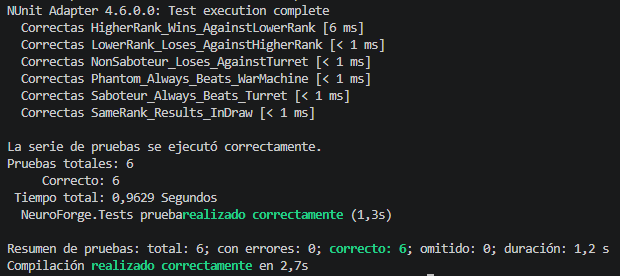
\includegraphics[width=\textwidth]{../Imagenes/nunit_results}
	\caption{Resultado de la ejecución de las pruebas unitarias con NUnit.}
	\label{fig:nunit_results}
\end{figure}